\subsection{Subgraph and Subdivision}
\begin{definition}
    Subgraphs are subsets of vertices and egdes of some original graphs
\end{definition}
\begin{center}
    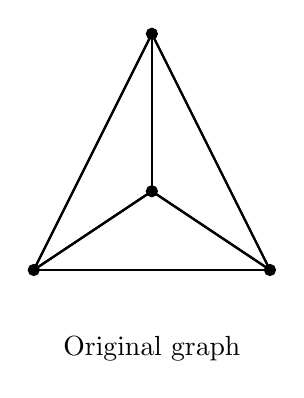
\begin{tikzpicture}
        \foreach \x/\y in {0/0, 1.5/1, 3/0, 1.5/3} {
                \filldraw[black] (\x,\y) circle (2pt);
                \foreach \z/\t in {0/0, 1.5/1, 3/0, 1.5/3} {
                        \draw[black, thick] (\x,\y) -- (\z,\t);
                    }
            }
        \node at (1.5,-1,0) {Original graph};
    \end{tikzpicture}
\end{center}

\begin{center}
    \begin{tikzpicture}
        \filldraw[black] (0,0) circle (2pt);
        \filldraw[black] (1.5,3) circle (2pt);
        \filldraw[black] (3,0) circle (2pt);
        \draw[black, thick] (0,0) -- (1.5,3);

        \filldraw[black] (7,0) circle (2pt);
        \filldraw[black] (8.5,3) circle (2pt);
        \filldraw[black] (10,0) circle (2pt);
        \draw[black, thick] (7,0) -- (8.5,3);
        \draw[black, thick] (10,0) -- (8.5,3);
        \draw[black, thick] (10,0) -- (7,0);

        \filldraw[black] (14,0) circle (2pt);
        \filldraw[black] (15.5,3) circle (2pt);
        \filldraw[black] (17,0) circle (2pt);
        \filldraw[black] (15.5,1) circle (2pt);
        \draw[black, thick] (14,0) -- (15.5,3);
        \draw[black, thick] (14,0) -- (15.5,1);
        \draw[black, thick] (15.5,3) -- (15.5,1);
        \draw[black, thick] (17,0) -- (15.5,3);
        \node at (8.5, -1, 0) {3 Subgraphs};
    \end{tikzpicture}
\end{center}

\begin{corollary}
    If graph is planar then all subgraphs are planar
\end{corollary}

\begin{proof}
    Contradiction
\end{proof}

\begin{definition}
    Subdivisions are obtained by replacing an edge with 2 edges connected by a new vertex
\end{definition}

\begin{proof}
\end{proof}

\begin{center}
    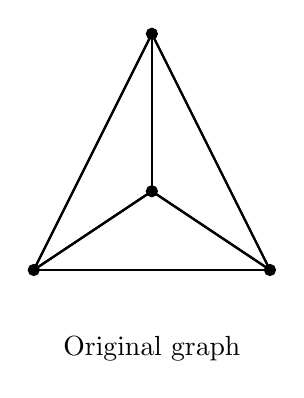
\begin{tikzpicture}
        \foreach \x/\y in {0/0, 1.5/1, 3/0, 1.5/3} {
                \filldraw[black] (\x,\y) circle (2pt);
                \foreach \z/\t in {0/0, 1.5/1, 3/0, 1.5/3} {
                        \draw[black, thick] (\x,\y) -- (\z,\t);
                    }
            }
        \node at (1.5,-1,0) {Original graph};
    \end{tikzpicture}
    \hspace{2cm}
    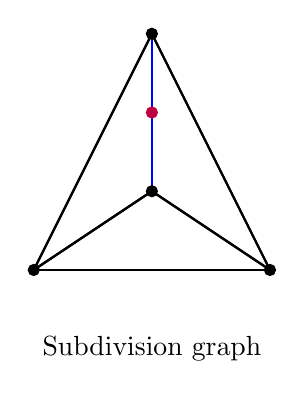
\begin{tikzpicture}
        \foreach \x/\y in {0/0, 1.5/1, 3/0, 1.5/3} {
                \foreach \z/\t in {0/0, 1.5/1, 3/0, 1.5/3} {
                        \draw[black, thick] (\x,\y) -- (\z,\t);
                    }
            }
        \node at (1.5,-1,0) {Subdivision graph};
        \draw[blue, thick] (1.5,1) -- (1.5,3);
        \filldraw[purple] (1.5,2) circle (2pt);
        \foreach \x/\y in {0/0, 1.5/1, 3/0, 1.5/3} {
                \filldraw[black] (\x,\y) circle (2pt);
            }
    \end{tikzpicture}
\end{center}

\begin{corollary}
    If some subdivision is planar then graph is planar
\end{corollary}
\begin{proof}
    Ai biết đâu.
\end{proof}
\begin{lemma}
    If graph is nonplanar then all subdivisions are nonplanar
\end{lemma}